\chapter{Einleitung}
Im folgenden wird die Umsetzung eines Programmes f�r die CoolSoft AG im Rahmen des Informationstechnik-Praktikums f�r den Studiengang Elektro- und Informationstechnik beschrieben.
\\
\\
Es wird als erstes auf die allgemeine Problemstellung eingegangen. Nachfolgend beschreiben wir dann besonderheiten unserer L�sung und Probleme die w�hrend des bearbeiten aufgetreten sind. Schlussendlich ist dann nat�rlich noch der komplette Code abgebidruckt.
\\
\\
In einem umfangreichen Praktikumspaket wurde der genaue Programmaufbau erl�utert, inklusive Klassendiagramm. F�r einzelne Programmteile wie zum Beispiel die Analyse und Tiefensuche wurde Pseudocode vorgegeben. Somit ging es im allgemeinen nur um die Realisation in C++.

\begin{figure}[h]
\centering
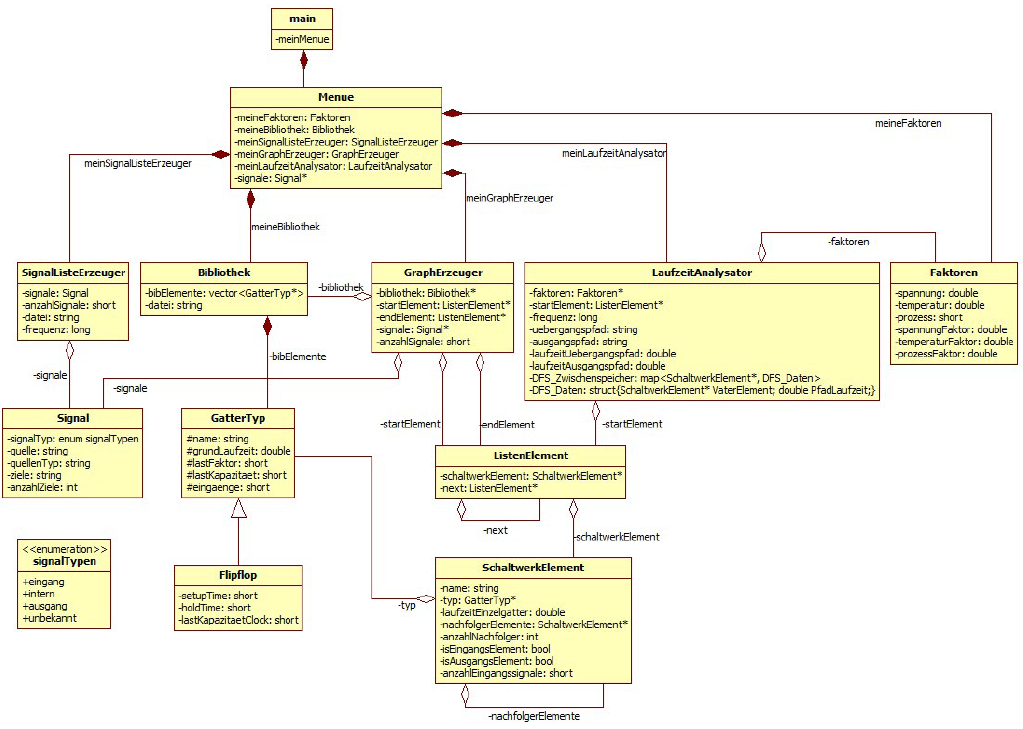
\includegraphics[width=\textwidth]{pictures/schema.png}
\caption{Klassendiagramm}
\end{figure}